% Materiais e Métodos
% Base: docs/proposta/4_Metodologia.tex, com os verbos no PASSADO e só o que foi
% efetivamente realizado. Acrescenta a subseção 3.4, do aplicativo desenvolvido, que a
% proposta não tinha. Retirado da proposta: alternativas tecnológicas descartadas, o
% cronograma e os resultados esperados.
%
% ESTA SEÇÃO ESTÁ COMPLETA — descreve o que foi feito, e tudo o que ela afirma já existe.

\chapter{Materiais e Métodos}\label{chap:metodologia}

\section{Caracterização da pesquisa}

A pesquisa caracteriza-se como descritiva e aplicada: estrutura um conjunto de critérios
técnicos já consolidados na literatura agronômica e aplica esse conhecimento na
construção e na avaliação de um artefato computacional \citep{Wazlawick2014}. Quanto ao
estilo de pesquisa em Computação, enquadra-se na apresentação de um produto.

\cite{Wazlawick2014} adverte que esse estilo exige cautela, pois a simples demonstração
de funcionamento tem baixa aceitação científica: é preciso comparar o que foi construído
com alguma referência. Por isso a avaliação não se limitou à demonstração. As saídas
foram confrontadas com um oráculo técnico --- os valores obtidos pela aplicação manual e
independente dos critérios do Manual \citep{ManualCalagem2016} --- e o sistema foi
posicionado frente às ferramentas discutidas no \cref{chap:revisao}.

\section{Escopo e fonte de conhecimento}

O escopo abrange as \textbf{61 culturas e grupos de culturas} para as quais o Manual
publica tabelas completas de adubação, organizadas em seis grupos: 21 de grãos, 18
hortaliças, 2 tubérculos, 17 frutíferas, erva-mate e 2 outras culturas comerciais
(cana-de-açúcar e tabaco). A contagem segue a organização do próprio Manual, em que
culturas que compartilham tabela --- melancia e melão, por exemplo --- contam como uma
entrada. Ficaram fora o arroz irrigado por alagamento, a mandioca, as espécies
florestais tolerantes à acidez e os grupos de forrageiras, palmeiras, medicinais e
ornamentais.

A \textbf{fonte técnica é única}: o Manual de Calagem e Adubação para os estados do RS e
de SC, 11\textsuperscript{a} edição \citep{ManualCalagem2016}. A base de conhecimento foi
transcrita manualmente pelo autor a partir da publicação, e a rastreabilidade de cada
tabela para o arquivo correspondente foi registrada em documento próprio do repositório.

\subsection{Controle sobre a transcrição}

A transcrição a partir do PDF revelou uma ameaça concreta à validade que exigiu controle
explícito. O PDF do Manual \textbf{não contém o caractere \textquotesingle$\leq$\textquotesingle{} na
camada de texto}: ele é desenhado como imagem embutida de aproximadamente
6~$\times$~6~pt, que nenhuma ferramenta de extração recupera. O comportamento é
inconsistente entre páginas --- ora o símbolo desaparece, ora é devolvido como sinal de
igualdade ---, de modo que um valor exato torna-se indistinguível de um valor com
qualificador.

O procedimento adotado combinou quatro controles: extração automática do texto;
detecção programática dos glifos ausentes como objetos de imagem, filtrados por tamanho,
e sua reinserção na posição correta; conferência visual de páginas rasterizadas por
amostragem e em toda célula de qualificador duvidoso; e testes automatizados de
invariantes sobre as tabelas resultantes, como a monotonicidade das doses por classe de
teor.

O mesmo artefato explica uma decisão de leitura registrada no trabalho: notas do Manual
que condicionam exceções a teores de cálcio e magnésio aparecem no texto extraído com
sinal de igualdade, e foram lidas como limites mínimos. A leitura sustenta-se em cinco
evidências convergentes, entre elas o fato de o operador \textquotesingle$<$\textquotesingle{}
da mesma frase sobreviver à extração --- o que localiza a perda nos glifos de
desigualdade não estrita --- e o próprio Anexo~1 do Manual aplicar a exceção como
limiar em exemplo resolvido.

Como controle adicional, os grupos de exigência de fósforo e potássio de cada cultura
foram transcritos \textbf{três vezes}, em momentos e por caminhos distintos, e as três
transcrições concordam integralmente. Um teste automatizado mantém essa concordância
travada. Cabe a ressalva, porém, de que isso é evidência de \emph{correção da
transcrição}, e não de correção agronômica dos critérios.

\section{Tecnologia e arquitetura}

O sistema foi implementado em \textbf{Python 3.12} com \textbf{Flask} para a camada web.
A base de conhecimento ficou em arquivos \textbf{JSON} validados por \textit{JSON
Schema}, carregados em tempo de execução. O sistema roda localmente, sem banco de dados,
sem autenticação e sem chamada de rede.

Duas decisões de arquitetura merecem registro. A primeira: o motor de inferência foi
escrito em \textbf{Python puro}, sem biblioteca externa de sistemas especialistas. A
decisão é metodológica --- um motor de terceiros introduziria uma camada de resolução de
conflitos cujo comportamento precisaria ser, ele próprio, verificado, enquanto o objetivo
é que cada decisão seja auditável linha a linha. A segunda: os módulos de domínio e de
motor \textbf{não importam Flask}, de modo que o núcleo é executável e testável por
linha de comando, independentemente da interface.

A \cref{fig:arquitetura} resume as camadas e a fronteira entre elas.

A arquitetura separa quatro camadas: \texttt{dominio}, com as entidades;
\texttt{conhecimento}, com o carregamento e a validação da base; \texttt{motor}, com as
regras; e \texttt{relatorio} e \texttt{web}, com a apresentação. O motor expõe um
\textbf{ponto de entrada único}, a função \texttt{gerar\_laudo}, pura e determinística:
as mesmas entradas produzem sempre o mesmo laudo e a mesma trilha.


\begin{figure}[htb]
\centering
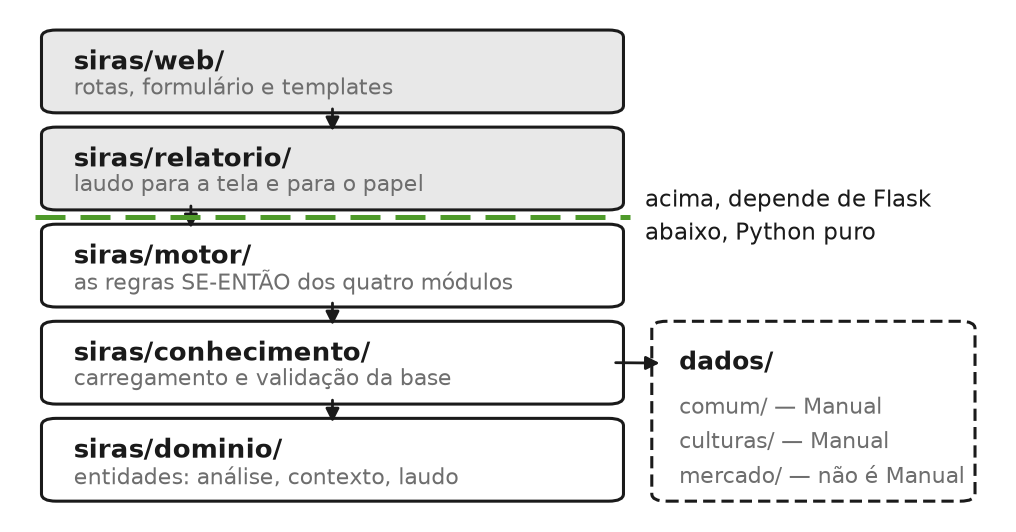
\includegraphics[width=0.95\textwidth]{fig/f1-arquitetura}
\caption{Camadas do SIRAS e a fronteira do Flask. O motor e o domínio não dependem da camada web, o que permite executá-los e testá-los por linha de comando, independentemente da interface.}
\label{fig:arquitetura}
\end{figure}

\subsection{Separação entre norma e dado de mercado}

Duas funcionalidades exigiram dados que o Manual não publica: a indicação de adubo
formulado e a caracterização de corretivos comerciais. Esses dados foram mantidos em
diretório separado da transcrição do Manual, e cada bloco declara a própria fonte e o
próprio estatuto --- lei vigente, convenção comercial herdada de norma revogada,
orientação do Manual ou ficha de fabricante.

A distinção não é formalidade de organização de arquivos. As faixas comerciais de PRNT
(A a D) e a classificação de corretivos por teor de óxido de magnésio, por exemplo, são
frequentemente apresentadas como exigência legal, mas têm origem em portaria revogada;
a norma vigente \citep{BrasilIN35_2006} fixa garantias mínimas e fatores de reatividade,
e não contém essas faixas. No sistema, elas estão rotuladas como convenção comercial histórica, e não
como norma.

\section{O aplicativo desenvolvido}\label{sec:aplicativo}

\subsection{Fluxo de uso}

O fluxo tem três telas. Na primeira, a pessoa escolhe entre os seis grupos e as 61
culturas. Na segunda, informa os dados da análise de solo; as variáveis condicionais que
cada cultura exige --- fase do pomar, ciclo da cana, tipo de tabaco, programa da
erva-mate --- aparecem por divulgação progressiva, lidas da base, de modo que a tela
nunca oferece uma opção que o motor recusaria. Enquanto a pessoa digita, um painel de
leitura ao vivo mostra em que classe cada teor caiu. Na terceira, o laudo.

A análise pode cobrir \textbf{vários talhões} num documento único, repetindo a análise
de solo por talhão e compartilhando cultura, manejo e corretivo. A área é opcional; se
informada para todos os talhões, o laudo acrescenta a quantidade total a comprar.


\begin{figure}[htb]
\centering
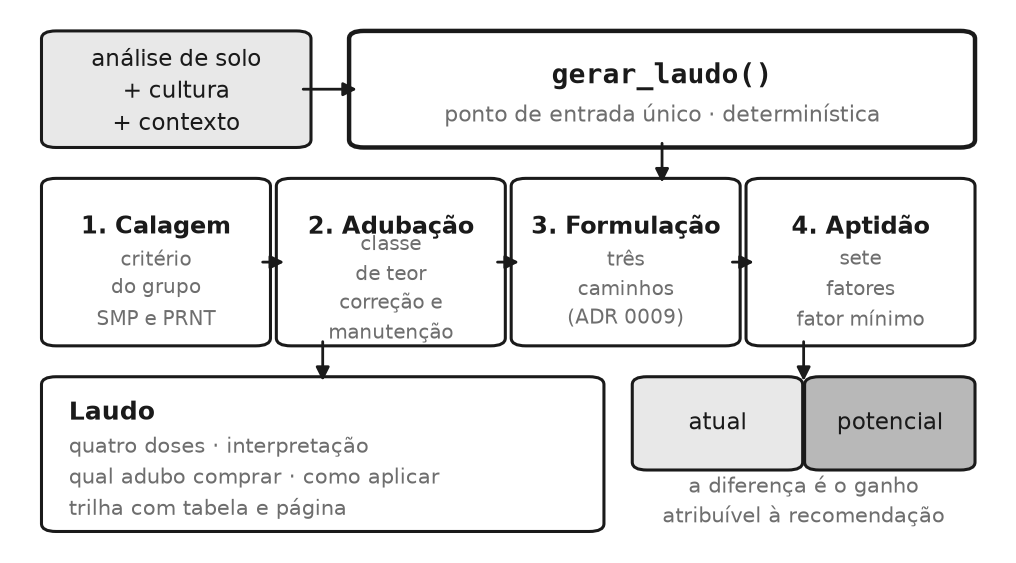
\includegraphics[width=0.95\textwidth]{fig/f2-fluxo}
\caption{Da análise de solo ao laudo, em uma passagem. A função \texttt{gerar\_laudo} é o ponto de entrada único e é determinística; os dois cenários de aptidão saem sempre juntos, porque é a diferença entre eles que quantifica o ganho atribuível à recomendação emitida.}
\label{fig:fluxo}
\end{figure}

\subsection{Módulos de recomendação}

O \textbf{módulo de calagem} resolve o critério aplicável à cultura e ao sistema de
manejo, consulta o índice SMP na Tabela 5.2 para o pH alvo do critério e converte a dose
pelo PRNT do corretivo informado. Trata os casos especiais do Manual: plantio direto
consolidado, em que a dose é um quarto da indicada para pH 6,0, aplicada em superfície e
limitada a 5~t/ha; solos de baixo poder tampão, em que equações polinomiais substituem a
tabela; e as culturas sem pH de referência, cuja calagem se decide por saturação por
bases.


\begin{figure}[htb]
\centering
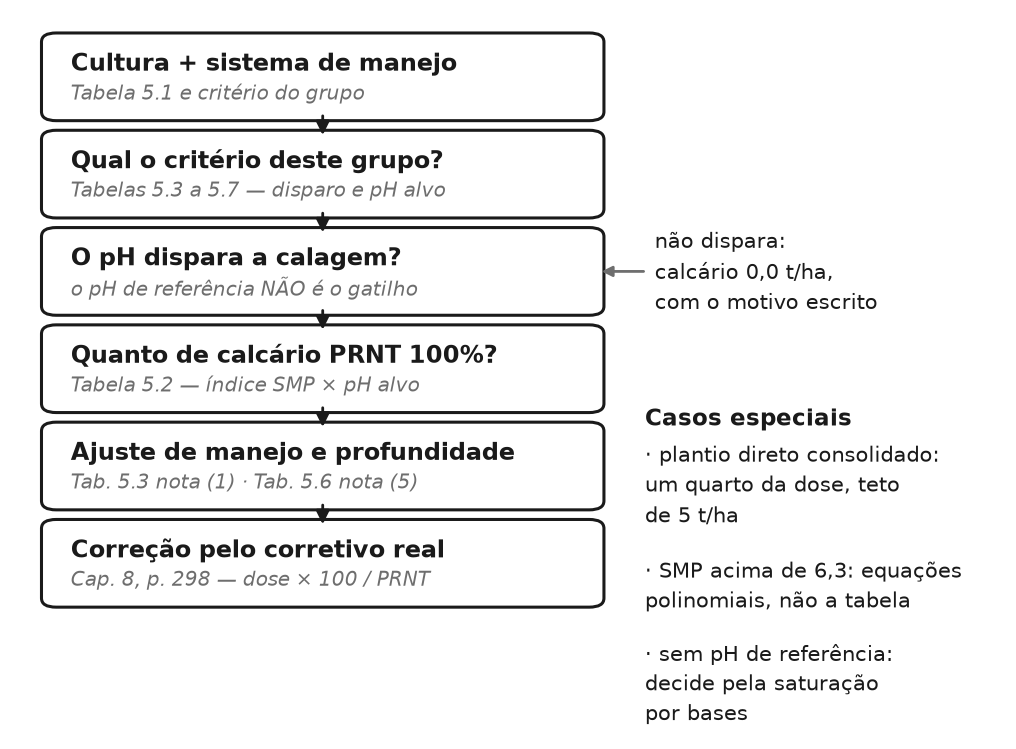
\includegraphics[width=0.88\textwidth]{fig/f3-calagem}
\caption{Decisão da dose de calcário, com a fonte de cada passo. A distinção entre o pH de referência e o critério de disparo é o ponto em que a aplicação manual do Manual mais erra.}
\label{fig:calagem}
\end{figure}

O \textbf{módulo de adubação} classifica o fósforo pela classe de teor de argila e o
potássio pela CTC a pH 7,0, segundo o grupo de exigência da cultura, e compõe as doses
de correção e manutenção. As culturas de grãos têm caminho próprio, por serem a exceção
do Manual --- publicam correção e manutenção em separado, com algoritmo por cultivo ---,
enquanto os outros cinco grupos compartilham um despacho parametrizado pelas variáveis
condicionais que cada um exige.

O \textbf{módulo de indicação de adubo formulado} converte a recomendação em produto,
pelo procedimento do Manual (\S8.3, p.~311): a dose da fórmula ancora-se no nutriente
mais deficiente no solo, que passa a ser atendido exatamente; o que faltar do outro é
completado com fertilizante simples, segundo as garantias da Tabela 8.4 --- hoje
atualizadas pela \cite{BrasilIN39_2018} ---; e o saldo de nitrogênio vai para cobertura. Entre as fórmulas do catálogo, a escolhida é a de menor
desvio relativo frente à recomendação, com desempate pela mais concentrada. O catálogo
de fórmulas é dado de mercado, declarado como tal no laudo, e o ranking é
\textbf{nutricional}: o Manual recomenda escolher pelo menor custo por unidade de NPK, e
o sistema não dispõe de preços.


\begin{figure}[htb]
\centering
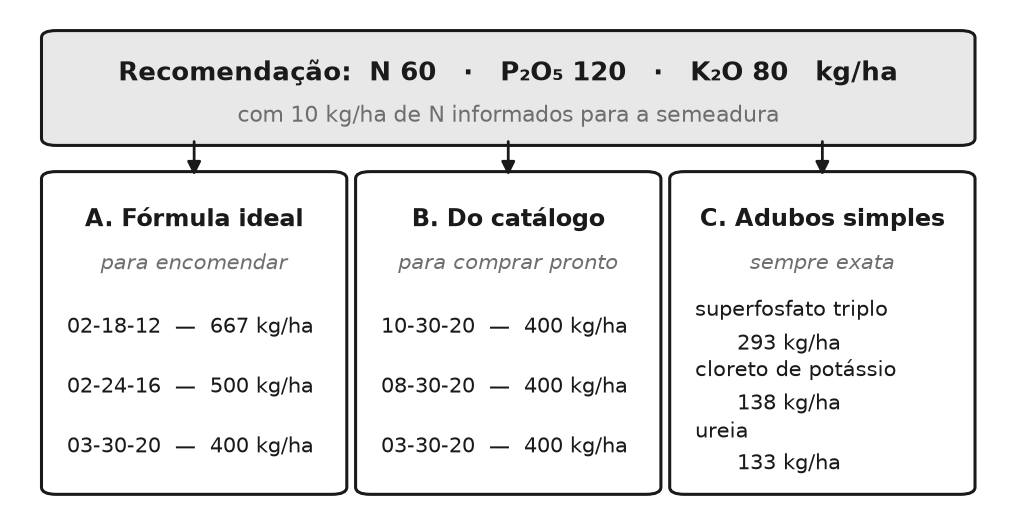
\includegraphics[width=0.95\textwidth]{fig/f4-formulacao}
\caption{Os três caminhos da formulação, resolvidos pelo próprio sistema sobre o exemplo publicado no Manual (§8.3, p.~311). A coluna A reproduz as três fórmulas e as doses que o Manual calcula. A coluna B mostra que o catálogo contém fórmulas reais de mesma proporção que o Manual não cita --- entre elas a 10-30-20, especificada em pregão público do Instituto Federal Farroupilha com entregas no Rio Grande do Sul, que vence por exigir menos massa total aplicada.}
\label{fig:formulacao}
\end{figure}

\begin{figure}[htb]
\centering
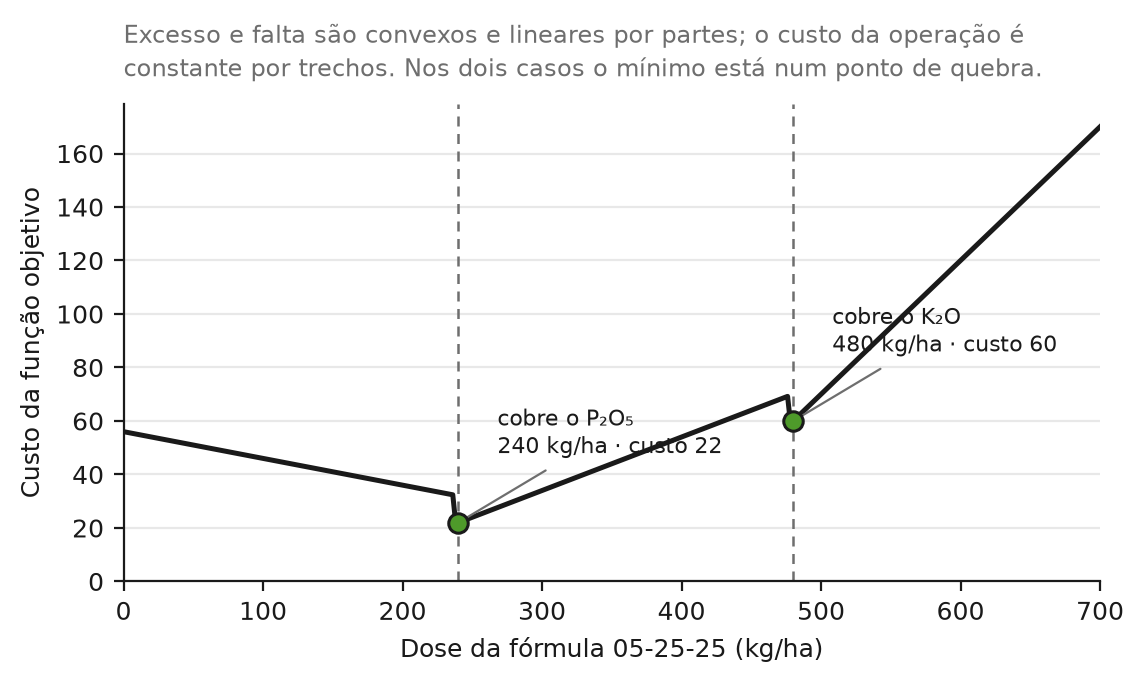
\includegraphics[width=0.95\textwidth]{fig/f5-pontos-de-quebra}
\caption{Custo em função da dose, para uma fórmula. Como o mínimo de uma função linear por partes convexa está em um ponto de quebra, basta avaliar as duas doses que atendem exatamente o P\textsubscript{2}O\textsubscript{5} e o K\textsubscript{2}O. A regra do Manual corresponde a um desses pontos.}
\label{fig:pontos-de-quebra}
\end{figure}

\subsection{Módulo de aptidão edáfica}

A estimativa de aptidão foi especificada em documento próprio --- um caderno de critérios
redigido \textbf{antes} da implementação e aprovado por escrito pelo orientador ---, sob
três princípios: nenhum limiar numérico criado pelo autor, com todo valor rastreando a
uma tabela do Manual ou a \cite{Sobral2015}; arquitetura derivada do sistema oficial, com
graus de limitação e regra do fator mínimo conforme \cite{RamalhoFilhoBeek1995} na
descrição de \cite{Hofig2015}; e toda decisão de julgamento do autor isolada, declarada
em apêndice e implementada como parâmetro configurável.

O módulo classifica a área em quatro níveis ordinais --- apta, apta com restrições,
restrita e inapta --- a partir de sete fatores de limitação, aplicando a regra do fator
mínimo. Dado ausente nunca é imputado por valor médio: gera classe indeterminada com
justificativa.

A saída traz \textbf{dois cenários}: o estado atual do solo e o estado projetado após as
correções que o próprio sistema acabou de recomendar. A diferença entre eles quantifica
o ganho atribuível à recomendação, e é o que integra os módulos --- emitir apenas um dos
dois perderia justamente a integração que distingue a solução.


\begin{figure}[htb]
\centering
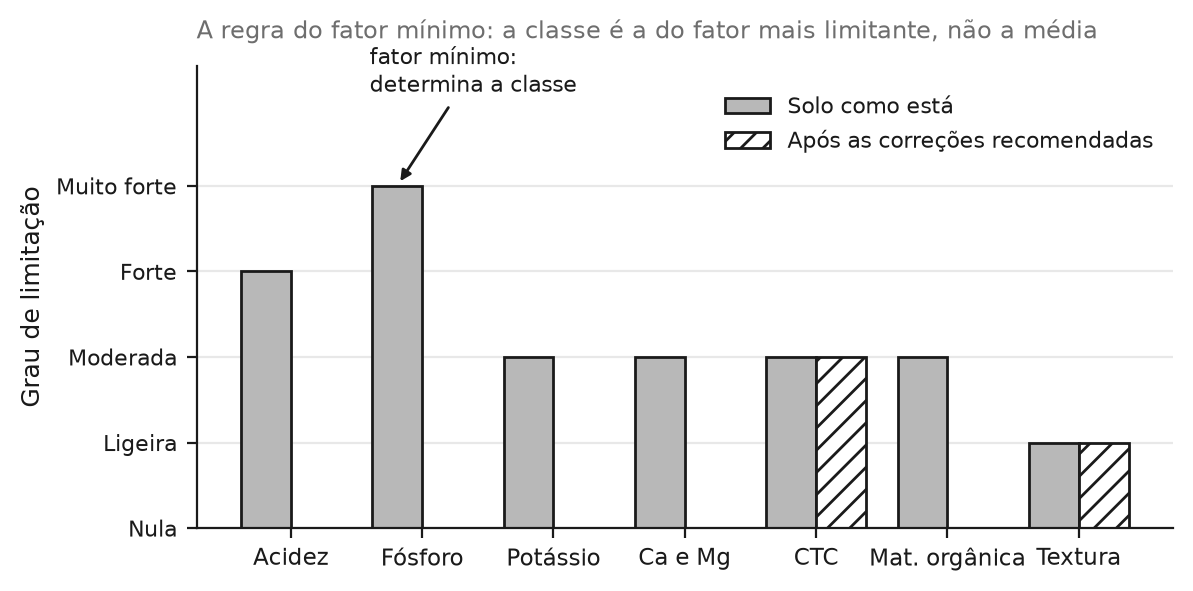
\includegraphics[width=0.95\textwidth]{fig/f6-aptidao}
\caption{Grau de limitação dos sete fatores, nos dois cenários, para uma análise real. A classe resulta do fator mais limitante, e não da média. Os fatores que a calagem e a adubação corrigem caem a zero no cenário projetado; CTC e textura permanecem, por serem limitações não corrigíveis em uma safra.}
\label{fig:aptidao}
\end{figure}

\subsection{Trilha de inferência}

Toda decisão do motor registra um passo contendo a regra aplicada, as entradas, a saída
e a fonte --- tabela e página do Manual. A trilha é impressa no laudo, agrupada por
módulo, e é o que permite a um terceiro conferir cada número sem acesso ao código. Essa
exigência é estrutural, e não opcional: em um documento que pode instruir projeto de
crédito rural, a recomendação sem procedência verificável tem pouco valor.

\section{Procedimento de avaliação}

A avaliação foi organizada em três dimensões.

\textbf{(i) Correção das saídas.} Um conjunto de casos de teste com oráculo calculado
manualmente pelo autor, a partir do Manual e sem consultar o código. Um caso é
considerado concordante quando \textbf{todas} as saídas declaradas na referência ---
necessidade de calcário e doses de N, P\textsubscript{2}O\textsubscript{5} e
K\textsubscript{2}O --- coincidem com a saída do sistema, admitida apenas tolerância de
arredondamento: uma casa decimal em t/ha para o calcário e números inteiros em kg/ha para
os nutrientes. Acertar três das quatro saídas é discordância, não acerto parcial. Apura-se
a proporção de casos concordantes, global e por grupo, com intervalo de confiança de 95\%
pelo método de \cite{Wilson1927} --- mais adequado que o intervalo normal para amostras
pequenas e proporções próximas de 1, por nunca produzir limites fora do intervalo
unitário. Casos discordantes são analisados individualmente, com a trilha de cada um.

Para a aptidão edáfica a verificação é de \textbf{conformidade}, e não de concordância:
mede se a implementação reproduz o caderno de critérios congelado, não se os critérios
estão agronomicamente corretos. O gabarito foi gerado aplicando o caderno manualmente e
é mantido em arquivo separado das entradas, de modo que o motor nunca o acessa.

\textbf{(ii) Comparação com ferramenta existente.} Natureza qualitativa, evidenciando
convergências, divergências e as funcionalidades que o SIRAS oferece e as demais não.

\textbf{(iii) Usabilidade.} Teste com usuários do público-alvo, descrito a seguir.

\subsection{Teste de usabilidade}

Participaram do teste \pendente{número final de participantes} profissionais e
estudantes do público-alvo --- agrônomos, técnicos agrícolas e estudantes concluintes de
agronomia ---, precedidos de um estudo-piloto com um participante que não integrou a
amostra.

Cada participante percorreu três roteiros em sessão única de aproximadamente 35 minutos:
(i)~demonstração conduzida pelo pesquisador sobre um cenário pronto, dando o primeiro
contato; (ii)~cenário fechado, entregue em ficha, executado pelo participante
\textbf{sozinho}; e (iii)~geração de um laudo \textbf{livre}, com cultura e dados de
escolha do próprio participante. Em (ii) e (iii) o pesquisador não auxiliou, devolvendo
as perguntas ao participante, pois cada intervenção suprimiria o registro de um problema
de usabilidade.

Concluída a sessão, e em momento separado, o participante respondeu a um
\textbf{questionário pós-teste estruturado pelas dez heurísticas de Nielsen}
\citep{Nielsen1994}, atribuindo a cada heurística uma nota de severidade de 0 a 4 e
descrevendo em texto livre as falhas e as telas em que ocorreram, seguido de quatro
perguntas abertas. Adotou-se esse instrumento em lugar do \textit{System Usability Scale}
\citep{Brooke1996} porque o SUS produz um escore único, ao passo que esta etapa precisava
produzir um diagnóstico acionável: a grade das heurísticas classifica cada problema pela
dimensão que ele viola e permite ordenar as correções por severidade. Perde-se a
comparabilidade com a literatura de escores SUS, o que se registra como limitação.

Cabe a distinção terminológica: \textbf{não se trata de avaliação heurística} no sentido
de \cite{NielsenMolich1990}, que designa a inspeção por especialistas em usabilidade,
sem usuários e sem tarefas. São usuários finais executando tarefas reais, e as notas ---
atribuídas por usuários a heurísticas, e não por avaliadores a problemas --- exprimem
percepção de gravidade, analisada por estatística descritiva, sem inferência. O
dimensionamento da amostra seguiu \cite{NielsenLandauer1993}.

A versão avaliada foi congelada antes da primeira sessão e mantida inalterada até a
última, de modo que todos os participantes avaliassem o mesmo sistema. Problemas
identificados durante a coleta foram anotados, não corrigidos. A etapa não requer
submissão a comitê de ética, e não houve termo de consentimento assinado: o participante
usou o sistema e respondeu ao formulário, que não coleta identificação direta.
